\documentclass[11pt]{article}
\usepackage[scaled=0.92]{helvet}
\usepackage{geometry}
\geometry{letterpaper,tmargin=1in,bmargin=1in,lmargin=1in,rmargin=1in}
\usepackage[parfill]{parskip} % Activate to begin paragraphs with an empty line rather than an indent %\usepackage{graphicx}
\usepackage{amsmath,amssymb, mathrsfs, dsfont}
\usepackage{tabularx}
\usepackage[font=footnotesize,labelfont=bf]{caption}
\usepackage{graphicx}
\usepackage{xcolor}
%\usepackage[linkbordercolor ={1 1 1} ]{hyperref}
%\usepackage[sf]{titlesec}
\usepackage{natbib}
\usepackage{../../Tianpei_Report}

%\usepackage{appendix}
%\usepackage{algorithm}
%\usepackage{algorithmic}

%\renewcommand{\algorithmicrequire}{\textbf{Input:}}
%\renewcommand{\algorithmicensure}{\textbf{Output:}}



\begin{document}
\title{Lecture 1: Smooth Manifolds}
\author{ Tianpei Xie}
\date{Oct. 14th., 2022}
\maketitle
\tableofcontents
\newpage
\section{Topological Manifolds}
\subsection{Definitions}
\begin{itemize}
\item \begin{definition}
Suppose $M$ is a \emph{\textbf{topological space}}. We say that $M$ is a \underline{\emph{\textbf{topological manifold}}} of \emph{dimension $n$} or a \emph{\textbf{topological $n$-manifold}} if it has the following properties:
\begin{enumerate}
\item $M$ is a \emph{\textbf{Hausdorff space}}: for every pair of distinct points $p, q \in M$, there are disjoint open subsets $U, V \subseteq M$ such that $p \in U$ and $q \in V$.
\item $M$ is \emph{\textbf{second-countable}}: there exists a \emph{\textbf{countable basis}} for the topology of $M$.
\item $M$ is \emph{\textbf{locally Euclidean of dimension}} $n$: each point of $M$ has a neighborhood that is \emph{\textbf{homeomorphic}} to an open subset of $\bR^n$. 
\end{enumerate}
\end{definition}

\item The third property means, more specifically, that for each $p \in M$ we can find
\begin{itemize}
\item an open subset $U \subseteq M$ containing $p$,
\item an open subset $\widehat{U}\subseteq \bR^n$, and
\item a \emph{homeomorphism} $\varphi: U\rightarrow \widehat{U}$.
\end{itemize}

\item It is important to note that every topological manifold has, by definition, a spe- cific, well-defined dimension.
\begin{theorem} (\textbf{Topological Invariance of Dimension}).\\
A nonempty $n$-dimensional topological manifold cannot be \textbf{homeomorphic} to an $m$-dimensional manifold unless $m = n$.
\end{theorem}

The dimension of a topological manifold $M$ is denoted as $\text{dim}\,M$.

\item The \emph{empty set} satisfies the definition of a topological $n$-manifold for every $n$. For the most part, we will ignore this special case.

\item The basic example of a topological $n$-manifold is $\bR^n$ itself. It is \emph{Hausdorff} because it is a \emph{metric space}, and it is \emph{second-countable} because the set of all open balls with \emph{rational centers} and \emph{rational radii} is a \emph{countable basis} for its topology.
\end{itemize}



\subsection{Coordinate Charts}
\begin{itemize}
\begin{figure}
\begin{minipage}[t]{1\linewidth}
  \centering
  \centerline{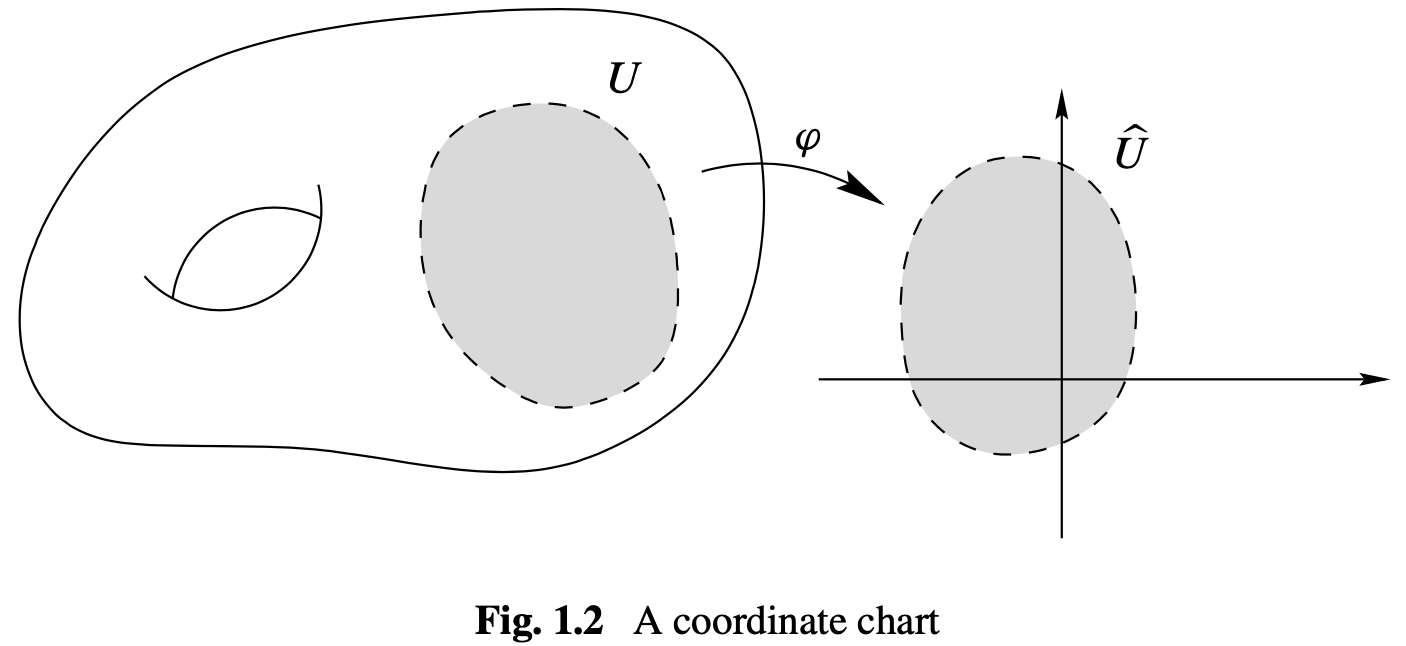
\includegraphics[scale = 0.45]{coordinate_chart.png}}
\end{minipage}
\caption{\footnotesize{\textbf{Coordinate chart \citep{lee2003introduction}}}}
\label{fig: coordinate_chart}
\end{figure}

\item \begin{definition}
Let $M$ be a \emph{topological n-manifold}. A \underline{\emph{\textbf{coordinate chart}}} (or just a \emph{chart}) on $M$ is a \emph{\textbf{pair}} $(U, \varphi)$, where $U$ is an open subset of $M$ and $\varphi: U \rightarrow \widehat{U}$ is a \emph{\textbf{homeomorphism}} from $U$ to an open subset $\widehat{U} = \varphi(U) \subseteq \bR^n$ (Fig. \ref{fig: coordinate_chart}). 

By definition of a topological manifold, each point $p \in M$ is contained in the \emph{domain} of some chart $(U, \varphi)$. If $\varphi(p) = 0$, we say that the chart is \emph{\textbf{centered at}} $p$. If $(U, \varphi)$ is any chart whose domain contains $p$, it is easy to obtain a new chart centered at $p$ by subtracting the constant vector $\varphi(p)$.
\end{definition}

\item \begin{definition}
Given a chart $(U, \varphi)$, we call the set $U$ a \emph{\textbf{coordinate domain}}, or a \emph{\textbf{coordinate neighborhood}} of each of its points. If, in addition, $\varphi(U)$ is an \emph{open ball} in $\bR^n$, then $U$ is called a \emph{\textbf{coordinate ball}}; if $\varphi(U)$ is an \emph{open cube}, $U$ is a \emph{\textbf{coordinate cube}}. The map $\varphi$ is called a \emph{\textbf{(local) coordinate map}}, and the \emph{component functions} $(x^1,\ldots, x^n)$ of $\varphi$, defined by $\varphi(p) = (x^1(p), \ldots, x^n(p))$, are called \emph{\textbf{local coordinates}} on $U$. 
\end{definition}
We sometimes write things such as ``$(U, \varphi)$ is a chart containing p" as shorthand for ``$(U, \varphi)$ is a chart whose domain $U$ contains p." If we wish to emphasize the coordinate function $(x^1,\ldots, x^n)$ instead of coordinate map $\varphi$, we sometimes denote the chart by $(U, (x^1,\ldots, x^n))$ or $(U, (x^i))$.
\end{itemize}

\subsection{Examples of Topological Manifolds}
\begin{itemize}
\item \begin{example} (\emph{\textbf{Graphs of Continuous Functions}}):\\
Let $U \subseteq \bR^n$ be an open subset, and let $f:U \rightarrow \bR^k$ be a \emph{continuous} function. The graph of $f$ is the subset of $R^n \times \bR^k$ defined by
\begin{align*}
\Gamma(f) &:= \set{ (x, y) \in R^n \times \bR^k: x\in U, \quad y = f(x) },
\end{align*} with the subspace topology. Let $\pi_1: \bR^n \times \bR^k \rightarrow \bR^n$ denote the \emph{projection} onto the
first factor, and let $\varphi: \Gamma(f) \rightarrow U$ be the restriction of $\pi_1$ to $\Gamma(f)$: 
\begin{align*}
\varphi(x, y) &= x,\quad \forall (x, y) \in \Gamma(f).
\end{align*} Because $\varphi$ is the restriction of a continuous map, it is continuous; and it is a homeomorphism because it has a continuous inverse given by $\varphi^{-1}(x) = (x, f(x))$. Thus $\Gamma(f)$ is a \emph{topological manifold of dimension $n$}.
\end{example}

\item \begin{example} (\emph{\textbf{Spheres}}):\\
For each integer $n \neq 0$, the unit $n$-sphere $\bS^n$ is \emph{Hausdorff} and \emph{second-countable} because it is a topological subspace of $\bR^{n+1}$. 

To show that it is \emph{locally Euclidean}, for each index $i = 1,\ldots,n+1$,  let $U_{i}^{+}$ denote the subset of $\bR^{n+1}$ where the $i$-th coordinate is positive:
\begin{align*}
U_{i}^{+} &= \set{(x^1, \ldots, x^{n+1}) \in \bR^{n+1}: x^i > 0 }.
\end{align*} Similarly, $U_{i}^{-}$ is the set where $x^i < 0$.

Let $f: \mathbb{B}^n \rightarrow \bR$ be the continuous function:
\begin{align*}
f(u) &= \sqrt{1 - \norm{u}{2}^2}
\end{align*}
Then for each  $i = 1,\ldots,n+1$, it is easy to check that $U_{i}^{+} \cap \bS^{n}$ is the graph of the function
\begin{align*}
x^{i} &= f(x^1, \ldots, x^{i-1}, \hat{x}^{i}, x^{i+1}, \ldots, x^{n+1})
\end{align*} where $\hat{x}^{i}$ indicates that $x^{i}$ is \emph{omitted}. Similarly, $U_{i}^{-} \cap \bS^{n}$ is the graph of the function
\begin{align*}
x^{i} &= -f(x^1, \ldots, x^{i-1}, \hat{x}^{i}, x^{i+1}, \ldots, x^{n+1}).
\end{align*}
Thus, each subset $U_{i}^{\pm} \cap\, \bS^{n}$ is \emph{locally Euclidean} of dimension $n$, and the maps $\varphi_{i}^{\pm}: U_{i}^{\pm} \cap \,\bS^{n} \rightarrow \mathbb{B}^{n}$ given by
\begin{align*}
\varphi_{i}^{\pm}(x^1, \ldots, x^{n+1}) &= (x^1, \ldots, x^{i-1}, \hat{x}^{i}, x^{i+1}, \ldots, x^{n+1})
\end{align*} are graph coordinates for $\bS^n$. Since each point of $\bS^n$ is in the domain of at least one
of these $2n + 2$ charts, $\bS^n$ is a \emph{topological n-manifold}.
\end{example}



\begin{figure}
\begin{minipage}[t]{0.5\linewidth}
  \centering
  \centerline{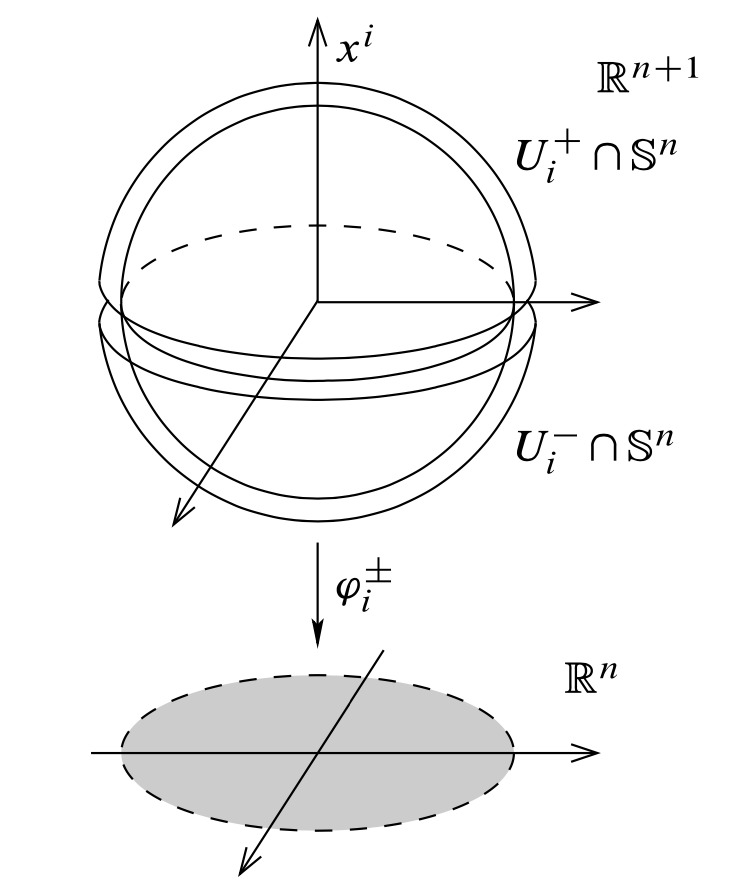
\includegraphics[scale = 0.4]{chart_sphere.png}}
\end{minipage}
\begin{minipage}[t]{0.5\linewidth}
  \centering
  \centerline{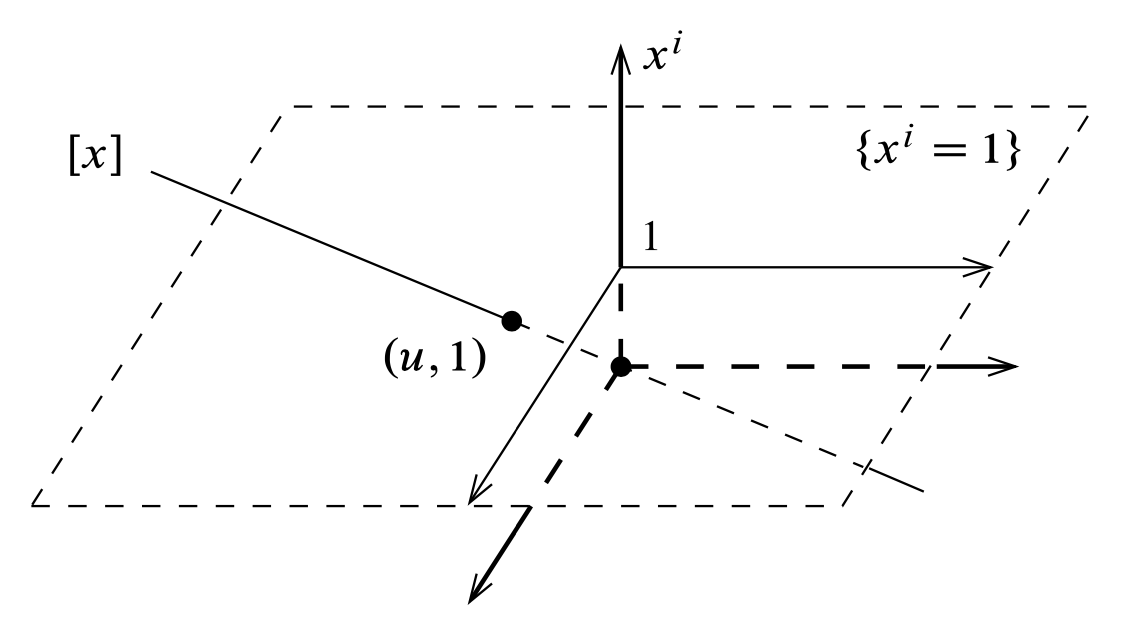
\includegraphics[scale = 0.4]{chart_projective.png}}
\end{minipage}
\caption{\footnotesize{\textbf{Coordinate chart for sphere (left) and projective space (right) \citep{lee2003introduction}}}}
\label{fig: coordinate_chart_sphere_projective}
\end{figure}

\item \begin{example} (\emph{\textbf{Projective Spaces}}).\\
The \emph{\textbf{$n$-dimensional real projective space}}, denoted by $\bR\bP^n$ (or sometimes just $\bP^n$), is defined as \emph{t\textbf{he set of $1$-dimensional linear subspaces}} of $\bR^{n+1}$, with the \emph{\textbf{quotient topology}} determined by the \emph{natural map} $\pi: \bR^{n+1} \setminus \set{0} \rightarrow \bR\bP^n$ sending each point $x \in  \bR^{n+1} \setminus \set{0}$ to the subspace spanned by $x$. The $2$-dimensional \emph{projective space} $\bR\bP^2$ is called the \emph{\textbf{projective plane}}. For any point $x \in  \bR^{n+1} \setminus \set{0}$, let $[x] = \pi(x) \in \bR\bP^2$ denote the line spanned by $x$.

For each $i=1,\ldots, n+1$, let $\tilde{U}_i \subseteq  \bR^{n+1} \setminus \set{0}$ be the set where $x^i \neq 0$, and let $U_i = \pi(\tilde{U}_i) \subseteq \bR\bP^n$. Since $\tilde{U}_i$ is a saturated open subset, $U_i$ is open and
$\pi \big|_{\tilde{U}_i}: \tilde{U}_i \rightarrow U_i$ is a \emph{quotient map}. Define a map $\varphi_i: U_i \rightarrow \bR^n$
by
\begin{align*}
\varphi_{i}[x^1, \ldots, x^{n+1}] &= \paren{\frac{x^1}{x^{i}}, \ldots, \frac{x^{i-1}}{x^{i}}, \frac{x^{i+1}}{x^{i}},\ldots, \frac{x^{n+1}}{x^{i}}}
\end{align*}

This map is well defined because its value is unchanged by multiplying $x$ by a nonzero constant. Because $\varphi_i \circ \pi$ is continuous, $\varphi_i$ is continuous by the characteristic property of quotient maps. In fact, $\varphi_i$ is a \emph{homeomorphism}, because it has a \emph{continuous inverse} given by
\begin{align*}
\varphi_{i}[u^1, \ldots, u^{n}] &= \paren{u^1, \ldots, u^{i-1}, 1, u^{i+1}, \ldots, u^{n}}.
\end{align*} 
Geometrically, $\varphi([x]) = u$ means $(u, 1)$ is the point in $\bR^{n+1}$ where the line $[x]$ intersects the affine hyperplane where $x^i = 1$.  Because the sets $U_1,\ldots, U_{n+1}$ cover $\bR\bP^n$, this shows that $\bR\bP^n$ is \emph{locally Euclidean of dimension $n$}. The \emph{Hausdorff} and \emph{second-countability} properties are left as exercises.
\end{example}

\item \begin{example} (\emph{\textbf{Product Manifolds}}).\\
 Suppose $M_1 ,\ldots, M_k$ are topological manifolds of dimensions $n_1,\ldots,n_k$, respectively. The product space $M_1 \times \ldots \times M_k$ is shown to be a \emph{topological manifold of dimension} $n_1 + \ldots + n_k$ as follows. It is Hausdorff and second-countable, so only the locally Euclidean property needs to be checked. 
 
Given any point $(p_1, \ldots, p_k) \in  M_1 \times \ldots \times M_k$,we can choose a coordinate chart $(U_i, \varphi_i)$ for each $M_i$ with $p_i \in U_i$. The product map:
\begin{align*}
\varphi_1\times \ldots \times \varphi_{k}: U_1 \times \ldots \times U_k \rightarrow \bR^{n_1 + \ldots + n_k}
\end{align*} is a homeomorphism onto its image, which is a product open subset of $\bR^{n_1 + \ldots + n_k}$. Thus, $M_1 \times \ldots \times M_k$ is a \emph{topological manifold of dimension} $n_1 + \ldots + n_k$, with charts of the form $(U_1 \times \ldots \times U_k, \varphi_1\times \ldots \times \varphi_{k})$.
\end{example}

\item \begin{example} (\emph{\textbf{Tori}}).\\
 For a positive integer $n$, the \emph{\textbf{n-torus}} (plural: \emph{\textbf{tori}}) is the product space $\mathbb{T}^n = \bS^1 \times \ldots \times \bS^1$. By the discussion above, it is a \emph{topological n-manifold}. (The \emph{$2$-torus} is usually called simply the \emph{\textbf{torus}}.)
 \end{example}
\end{itemize}

\subsection{Topological Properties of Manifolds}
\begin{itemize}
\item As topological spaces go, manifolds are quite special, because they share so many important properties with Euclidean spaces. 

\item \begin{lemma}
Every topological manifold has a countable basis of \textbf{precompact} coordinate balls.
\end{lemma}
\end{itemize}

\subsubsection{Connectivity}
\begin{itemize}
\item \begin{definition}
Recall that a topological space $X$ is
\begin{itemize}
\item \emph{\textbf{connected}} if there do not exist two disjoint, nonempty, open subsets of $X$ whose union is $X$;
\item \emph{\textbf{path-connected}} if every pair of points in $X$ can be joined by a path in $X$, and
\item \emph{\textbf{locally path-connected}} if $X$ has a basis of path-connected open subsets.
\end{itemize}
\end{definition}

\item \begin{definition}
A \emph{\textbf{maximal connected subset}} of $X$ (i.e., a connected subset that is not properly contained in any larger connected subset) is called a \emph{\textbf{component}} (or connected component) of $X$.
\end{definition}

\item The following proposition shows that connectivity and path connectivity \textbf{coincide} for manifolds.
\begin{proposition}
Let $M$ be a topological manifold.
\begin{enumerate}
\item $M$ is \textbf{locally path-connected}.
\item $M$ is connected \textbf{if and only} if it is path-connected.
\item The components of $M$ are the same as its path components.
\item $M$ has \textbf{countably} many \textbf{components}, each of which is an open subset of $M$ and a \textbf{connected} topological manifold.
\end{enumerate}
\end{proposition}
\end{itemize}

\subsubsection{Local Compactness and Paracompactness}
\begin{itemize}
\item \begin{definition}
A topological space $X$ is said to be \emph{\textbf{compact}} if every open cover of $X$ has a \emph{\textbf{finite} subcover}. A \emph{\textbf{compact subset}} of a topological space is one that is a compact space in the subspace topology. 
\end{definition}

\item \begin{definition}
A topological space $X$ is said to be \emph{\textbf{locally compact}} if every point has a neighborhood contained in a \emph{compact subset} of $X$. 

A subset of $X$ is said to be \emph{\textbf{precompact}} in $X$ if its \emph{\textbf{closure}} in $X$ is \emph{compact}.
\end{definition}

\item For a \emph{\textbf{Hausdorff space}} $X$, show that the following are equivalent:
\begin{enumerate}
\item $X$ is \emph{\textbf{locally compact}}.
\item Each point of $X$ has a \emph{precompact} neighborhood. 
\item $X$ has a basis of \emph{precompact} open subsets.
\end{enumerate}

\item 
\begin{proposition} (\textbf{Manifolds Are Locally Compact}).\\
Every topological manifold is \textbf{locally compact}.
\end{proposition}

\item Let $M$ be a topological space. A collection $\cX$ of subsets of $M$ is said to be \emph{\textbf{locally finite}} if each point of $M$ has a neighborhood that \emph{intersects} at most finitely many of the sets in $X$. Given a cover $\cU$ of $M$; another cover $\cV$ is called a \emph{\textbf{refinement}} of $\cU$ if for each $V \in \cV$ there exists some $U \in \cU$ such that $\cV \subset \cU$. We say that $M$ is \emph{\textbf{paracompact}} if every open cover of $M$ admits an open, locally finite refinement.

\item \begin{lemma}
Suppose $\cX$ is a locally finite collection of subsets of a topological space $M$.
\begin{enumerate}
\item The collection $\set{\overline{X}: X \in \cX}$ is also locally finite.
\item $\overline{\bigcup_{X \in \cX}\,X} = \bigcup_{X \in \cX}\,\overline{X}$.
\end{enumerate}
\end{lemma}

\item \begin{theorem} (\textbf{Manifolds Are Paracompact}).\\
Every topological manifold is \textbf{paracompact}. In fact, given a topological manifold $M$, an open cover $\cX$ of $M$, and any basis $\cB$ for the topology of $M$, there exists a \textbf{countable}, \textbf{locally finite open refinement} of $\cX$ consisting of elements of $\cB$.
\end{theorem}
\end{itemize}

%\subsubsection{Fundamental Groups of Manifolds}
%\begin{itemize}
%\item \begin{definition}
%If $X$ and $Y$ are topological spaces and $F_0,\, F_1: X \rightarrow Y$ are \emph{continuous} maps, a \emph{\textbf{homotopy}} from $F_0$ to $F_1$ is a \emph{continuous} map $H: X \times I \rightarrow Y$ satisfying
%\begin{align*}
%H(x, 0) &= F_0(x)\\
%H(x, 1) &= F_1(x)
%\end{align*} for all $x \in X$.
%
%If there exists a homotopy from $F_0$ to $F_1$,we say that $F_0$ and $F_1$ are \emph{\textbf{homotopic}}, and write $F_0 \simeq F_1$. If the homotopy satisfies $H(x, t) = F_0(x) = F_1(x)$ for all $t \in I$ and all $x$ in some subset $A \subseteq X$, the maps $F_0$ and $F_1$ are said to be \emph{\textbf{homotopic}} relative to $A$. Both "\emph{homotopic}" and "\emph{homotopic relative to $A$}" are \emph{\textbf{equivalence relations}} on the set of \emph{all continuous maps} from $X$ to $Y$.
%\end{definition}
%
%\item The most important application of homotopies is to paths. Suppose $X$ is a topological space. Two paths $f_0, f_1: I \rightarrow X$ are said to be \emph{\textbf{path-homotopic}}, denoted symbolically by $f_0 \sim f_1$, if they are \emph{homotopic} relative to $\set{0, 1}$. Explicitly, this means that there is a continuous map $H: I \times I \rightarrow X$ satisfying
%\begin{align*}
%H(s, 0) &= f_0(s), \quad s\in I \\
%H(s, 1) &= f_1(s), \\
%H(0, t) &= f_0(0) = f_1(0), \quad t\in I \\
%H(1, t) &= f_0(1) = f_1(1),
%\end{align*} 
%For any given points $p, q \in X$, \emph{path homotopy} is an \emph{\textbf{equivalence relation}} on the set of all paths from $p$ to $q$. The equivalence class of a path $f$ is called its \emph{\textbf{path class}}, and is denoted by $[f]$.
%
%\item \begin{definition}
%If $X$ is a topological space and $q$ is a point in $X$, \emph{\textbf{a loop}} in $X$ based at $q$ is a \emph{path} in $X$ from $q$ to $q$, that is, a \emph{continuous map} $f: I \rightarrow X$ such that $f(0) = f(1)= q$. The set of \emph{\textbf{path classes}} of loops based at $q$ is denoted by $\pi_1(X, q)$. Equipped with the product described above, it is a \emph{\textbf{group}}, called the \emph{\textbf{fundamental group}} of $X$ based at $q$. The \emph{identity element} of this group is the path class of the constant path $c_{q}(s) = q$, and the inverse of $[f]$ is the path class of the \emph{\textbf{reverse path}} $\overline{f}(s) =  f(1- s)$.
%\end{definition}
%
%\item \begin{theorem}
%The fundamental group of a topological manifold is \textbf{countable}.
%\end{theorem}
%\end{itemize}

\section{Smooth Structures}
\subsection{Definitions}
\begin{itemize}
\item To make sense of derivatives of real-valued functions, curves, or maps between manifolds, we need to introduce a new kind of manifold called a \emph{smooth manifold}.

\item \begin{definition}
If $U$ and $V$ are open subsets of Euclidean spaces $\bR^n$ and $\bR^m$, respectively, a function $F: U \rightarrow V$ is said to be \emph{\textbf{smooth}} (or $\cC^{\infty}$ , or \emph{infinitely differentiable}) if each of its component functions has continuous partial derivatives of \emph{all orders}. If in addition $F$ is \emph{bijective} and has a \emph{\textbf{smooth inverse map}}, it is called a \underline{\emph{\textbf{diffeomorphism}}}. A \emph{diffeomorphism} is, in particular, a \emph{homeomorphism}.
\end{definition}

\begin{figure}
\begin{minipage}[t]{1\linewidth}
  \centering
  \centerline{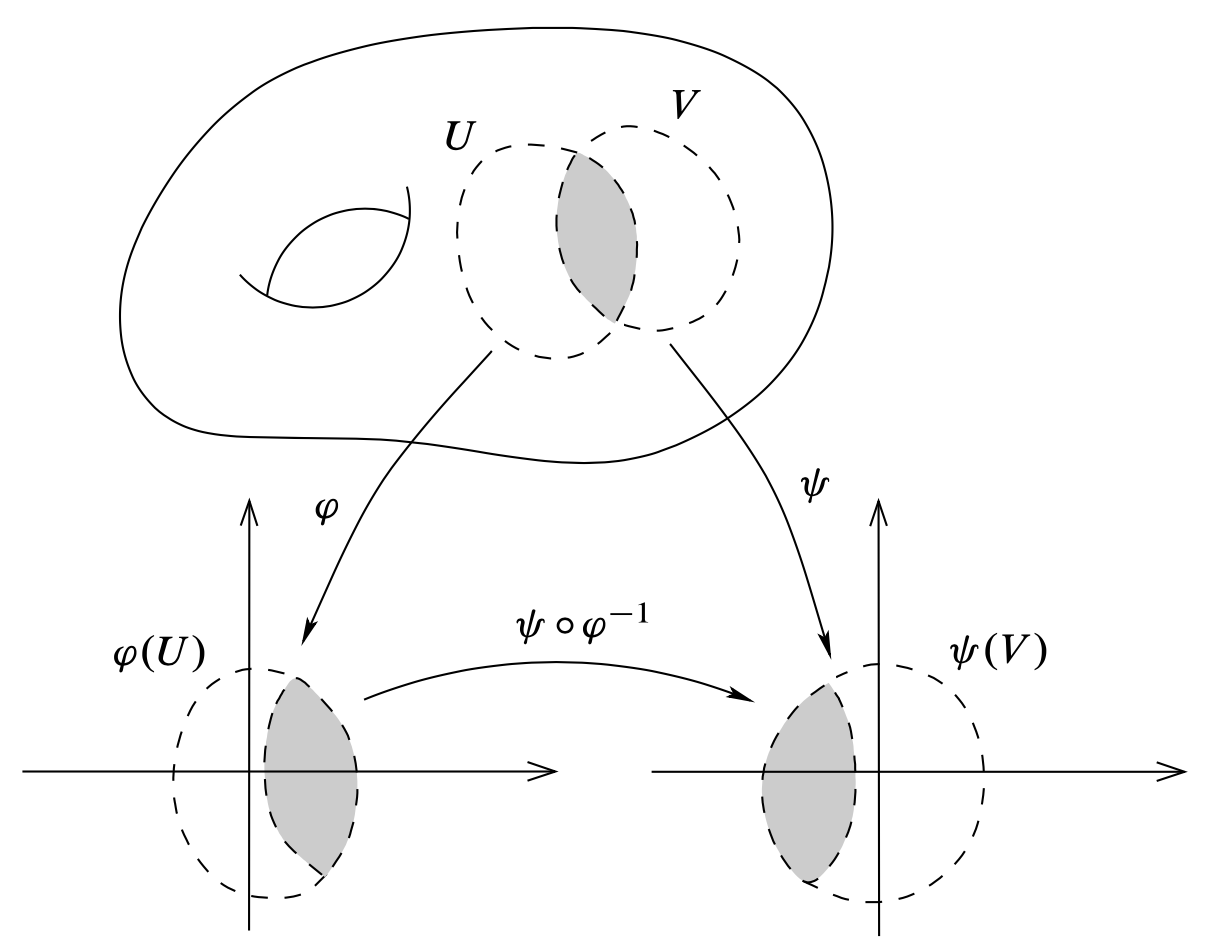
\includegraphics[scale = 0.4]{transition_map.png}}
\end{minipage}
\caption{\footnotesize{\textbf{A transition map \citep{lee2003introduction}}}}
\label{fig: transition_map}
\end{figure}


\item \begin{definition}
Let $M$ be a topological $n$-manifold. If $(U, \varphi)$, $(V, \psi)$ are two charts such that $U \cap V \neq \emptyset$, the composite map $\psi \circ \varphi^{-1}: \varphi(U \cap V ) \rightarrow \psi(U \cap V)$ is called the \emph{\textbf{transition map}} from $\varphi$ to $\psi$ (Fig. \ref{fig: transition_map}). It is a \emph{composition} of \emph{homeomorphisms}, and is therefore itself a \emph{homeomorphism}. Two charts $(U, \varphi)$ and $(V, \psi)$ are said to be \emph{\textbf{smoothly compatible}} if either $U \cap V = \emptyset$ or the transition map $\psi \circ \varphi^{-1}$ is a \emph{\textbf{diffeomorphism}}. Since $\varphi(U \cap V )$ and $\psi(U \cap V ) $ are open subsets of $\bR^n$, smoothness of this map is to be interpreted in the ordinary sense of having continuous partial derivatives of all orders.
\end{definition}

\item \begin{definition}
We define an \emph{\textbf{atlas}} for $M$ to be a collection of charts whose domains cover $M$. An atlas $\mathcal{A}$ is called a \emph{\textbf{smooth atlas}} if any two charts in $\mathcal{A}$ are \emph{smoothly compatible} with each other.
\end{definition}

To show that an atlas is smooth, we need only verify that each transition map $\psi \circ \varphi^{-1}$ is smooth whenever $(U, \varphi)$ and $(V, \psi)$ are charts in $\cA$. Given two particular charts $(U, \varphi)$ and $(V, \psi)$, it is often easiest to show that they are smoothly compatible by verifying that $\psi \circ \varphi^{-1}$ is smooth and injective with nonsingular Jacobian at each point.

\item \begin{definition}
A \emph{smooth atlas} $\cA$ on $M$ is \emph{\textbf{maximal}} if it is not properly contained in \emph{any larger smooth atlas}. This just means that any chart that is \emph{smoothly compatible} with \emph{every chart} in $\cA$ is already in $\cA$. (Such a smooth atlas is also said to be \emph{\textbf{complete}}.)
\end{definition}

\item 
\begin{definition}
If $M$ is a topological manifold, a \underline{\emph{\textbf{smooth structure}}} on $M$ is a \emph{maximal smooth atlas}. A \underline{\emph{\textbf{smooth manifold}}} is a pair $(M, \cA)$, where $M$ is a topological manifold and $\cA$ is a \emph{smooth structure} on $M$.

When the smooth structure is understood, we usually omit mention of it and just say ``\emph{$M$ is a smooth manifold.}" Smooth structures are also called \emph{\textbf{differentiable structures}} or \textbf{\emph{$\cC^{\infty}$ structures}} by some authors. We also use the term \emph{\textbf{smooth manifold structure}} to mean a manifold topology together with a smooth structure.
\end{definition}

\item In fact, a given topological manifold may have many different smooth structures. On the other hand, it is not always possible to find a smooth structure on a given topological manifold: there exist topological manifolds that admit no smooth structures at all.

\item It is generally not very convenient to define a smooth structure by explicitly describing a maximal smooth atlas, because such an atlas contains very many charts. Fortunately, we need only specify \emph{some} smooth atlas, as the next proposition shows.
\begin{proposition}
Let $M$ be a topological manifold.
\begin{enumerate}
\item Every smooth atlas $\cA$ for $M$ is contained in a \textbf{unique} maximal smooth atlas, called \textbf{the smooth structure determined by $\cA$}.
\item Two smooth atlases for $M$ determine the same smooth structure if and only if their union is a smooth atlas.
\end{enumerate}
\end{proposition}
For example, if a topological manifold $M$ can be covered by a single chart, the smooth compatibility condition is trivially satisfied, so \emph{any such chart automatically determines a smooth structure on} $M$.

\item if we replace the requirement that charts be smoothly compatible by the \emph{weaker} requirement that each transition map $\psi \circ \varphi^{-1}$ (and its inverse) be of $\cC^{k}$, we obtain the definition of a \emph{\textbf{$\cC^{k}$ structure}}. 

Similarly, if we require that each transition map be \emph{\textbf{real-analytic}} (i.e., expressible as a convergent power series in a neighborhood of each point), we obtain the definition of a \emph{\textbf{real-analytic structure}}, also called a \emph{\textbf{$\cC^{\omega}$ structure}}. 

If $M$ has even dimension $n = 2m$, we can identify $\bR^{2m}$ with $\bC^m$ and require that the transition maps be \emph{\textbf{complex-analytic}}, this determines a \emph{\textbf{complex-analytic structure}}. 

A manifold endowed with one of these structures is called a \emph{\textbf{$\cC^k$ manifold, real-analytic manifold, or complex manifold}}, respectively. (Note that a $\cC^0$ manifold is just a \emph{topological manifold}.)
\end{itemize}

\subsection{Local Coordinate Representations}
\begin{itemize}
\item \begin{definition}
If $M$ is a smooth manifold, any chart $(U, \varphi)$ contained in the given maximal smooth atlas is called a \emph{\textbf{smooth chart}}, and the corresponding coordinate map $\varphi$ is called a \emph{\textbf{smooth coordinate map}}. It is useful also to introduce the terms \emph{\textbf{smooth coordinate domain}} or \emph{\textbf{smooth coordinate neighborhood}} for the domain of a smooth coordinate chart. A \emph{\textbf{smooth coordinate ball}} means a \emph{smooth coordinate domain} whose image under a \emph{smooth coordinate map} is a ball in Euclidean space. A \emph{\textbf{smooth coordinate cube}} is defined similarly.
\end{definition}

\item It is often useful to restrict attention to coordinate balls whose closures sit nicely inside larger coordinate balls. 
\begin{definition}
We say a set $B \subseteq M$ is a \emph{\textbf{regular coordinate ball}} if there is a \emph{smooth coordinate ball} $B' \supseteq \overline{B}$ and a \emph{smooth coordinate map} $\varphi: B' \rightarrow \bR^n$ such that for some positive real numbers $r < r'$,
\begin{align*}
\varphi(B) = B_{r}(0), \quad \varphi(\overline{B}) = \overline{B_{r}}(0), \quad \varphi(B') = B_{r'}(0)
\end{align*}
\end{definition}

\item Because $\overline{B}$ is homeomorphic to $\overline{B_{r}}(0)$, it is compact, and thus every regular coordinate ball is \emph{precompact} in $M$.
\begin{proposition}
Every smooth manifold has a \textbf{countable} basis of \textbf{regular coordinate balls}.
\end{proposition}

\begin{figure}
\begin{minipage}[t]{1\linewidth}
  \centering
  \centerline{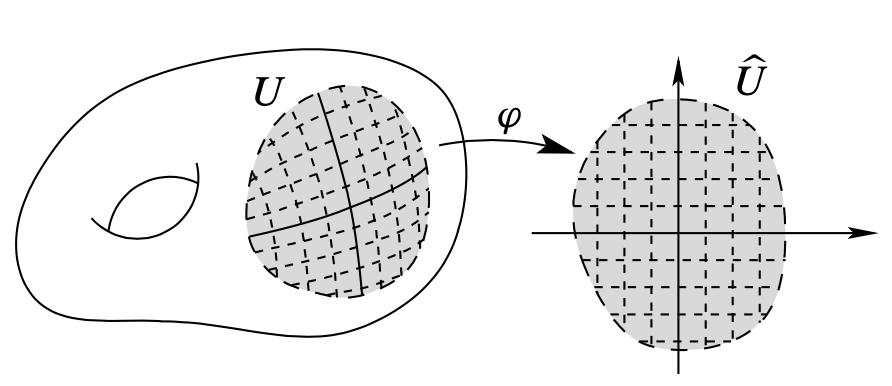
\includegraphics[scale = 0.5]{coordinate_grid.png}}
\end{minipage}
\caption{\footnotesize{\textbf{A local coordinate grid \citep{lee2003introduction}}}}
\label{fig: coordinate_grid}
\end{figure}

 
\item Here is how one usually thinks about \textbf{coordinate charts} on a smooth manifold. Once we choose a smooth chart $(U, \varphi)$ on $M$, the coordinate map $\varphi: U \rightarrow \widehat{U} \subset \bR^{n}$ can be thought of as giving a \emph{\textbf{temporary identification}} between $U$ and $\widehat{U}$. Using this identification, while we work in this chart, we can think of $U$ \emph{simultaneously} as an open subset of $M$ \emph{\textbf{and}} as an open subset of $\bR^n$. You can visualize this identification by thinking of a "grid" drawn on $U$ representing the \emph{preimages} of the coordinate lines under $\varphi$ (Fig. 1.8). Under this identification, we can represent a point $p \in U$ by its coordinates $(x^1,\ldots, x^n) = \varphi(p)$, and think of this $n$-tuple as \emph{being} the point p. We typically express this by saying ``\emph{$(x^1,\ldots, x^n) $ is \underline{\textbf{the (local) coordinate representation}} for $p$}" or ``\underline{\emph{$p = (x^1,\ldots, x^n)$ in local coordinates.}}"

Another way to look at it is that by means of our identification $U \leftrightarrow \widehat{U}$ , we can think of $\varphi$ as the \emph{identity map} and \emph{\textbf{suppress}} it from the notation. This takes a bit of getting used to, but the payoff is a huge simplification of the notation in many situations. You just need to remember that the identification is in general \emph{only local}, and depends heavily on the \emph{choice of coordinate chart}.

\item The fact that manifolds do not come with \emph{any predetermined choice of coordinates} is both a blessing and a curse.
\begin{itemize}
\item The \emph{\textbf{flexibility}} to choose coordinates more or less arbitrarily can be a big advantage in approaching problems in manifold theory.
\item But we pay for this flexibility by being obliged to ensure that \emph{\textbf{any objects we wish to define globally on a manifold are not dependent on a particular choice of coordinates}}.

There are generally two ways of doing this: either by writing down a \emph{coordinate-dependent definition} and then proving that the \emph{definition gives the same results in any coordinate chart}, or by writing down \emph{a definition that is manifestly coordinate-independent} (often called an \emph{\textbf{invariant definition}}).
\end{itemize}
\end{itemize}

\subsection{Examples of Smooth Manifolds}
\subsubsection{Examples}
\begin{itemize}
\item \begin{example} (\emph{\textbf{$0$-Dimensional Manifolds}}). \\
A topological manifold $M$ of dimension $0$ is just a \emph{\textbf{countable discrete space}}. For each point $p \in M$, the only neighborhood of $p$ that is \emph{homeomorphic} to an open subset of $\bR^0$ is $\set{p}$ itself, and there is exactly one coordinate map $\varphi: \set{p} \rightarrow \bR^0$. Thus, the set of all charts on $M$ trivially satisfies the smooth compatibility condition, and each $0$-dimensional manifold has a unique smooth structure.
\end{example}

\item \begin{example} (\emph{\textbf{Euclidean space}})\\
For each nonnegative integer $n$, the \emph{Euclidean space} $\bR^n$ is a \emph{smooth n-manifold} with the \emph{smooth structure} determined by the atlas consisting of the single chart $(\bR^n, \text{Id}_{\bR^n})$.
\end{example}

\item \begin{example} (\emph{\textbf{Finite-Dimensional Vector Spaces}})\\
Let $V$ be a \emph{finite-dimensional real vector space}. Any \emph{norm} on $V$ determines a topology, which is \emph{independent} of the choice of norm. With this topology, $V$ is a topological $n$-manifold, and has a \emph{natural smooth structure} defined as follows. Each (ordered) basis $(E_1,\ldots, E_n)$ for $V$ defines a \emph{\textbf{basis isomorphism}} $E: \bR^n \rightarrow V$ by
\begin{align*}
E(x) &= \sum_{i=1}^{n}x^{i}\,E_{i}.
\end{align*} This map is a \emph{homeomorphism}, so $(V, E^{-1})$ is a chart. If $(\widetilde{E}_1,\ldots, \widetilde{E}_n)$ is another basis, and the corresponding isomorphism $\widetilde{E}(x) = \sum_{j=1}^{n}x^{j}\,\widetilde{E}_{j}$, then there is some
invertible matrix $\mb{A}$ such that $E_i = \sum_{j}A_{i}^{j}\widetilde{E}_{j}$ for each $i$. The transition map between the two chars are given by $\widetilde{E}^{-1}\circ E(x) = \widetilde{x}$,  where $\widetilde{x} = (\widetilde{x}^{1},\ldots, \widetilde{x}^{n})$ is determined by
\begin{align*}
\sum_{j=1}^{n}x^{j}\,\widetilde{E}_{j} &= \sum_{i=1}^{n}x^{i}\,E_{i} = \sum_{i,j}x^{i}A_{i}^{j}\widetilde{E}_{j}.
\end{align*} It follows that $\widetilde{x}^{j} = \sum_{i,j}A_{i}^{j}x^{i}$. Thus, the map sending $x$ to $\widetilde{x}$ is an \emph{invertible linear map} and hence a \emph{diffeomorphism}, so any two such charts are \emph{smoothly compatible}. The collection of \emph{all such charts} thus defines \emph{a smooth structure}, called \textbf{\emph{the standard smooth structure}} on $V$.
\end{example}

\item \begin{example} (\emph{\textbf{Spaces of Matrices}}).\\
Let $M(m \times n, \bR)$ denote \emph{the set of $m \times n$ matrices with real entries}. Because it is a real vector space of dimension $mn$ under matrix addition and scalar multiplication, $M(m \times n, \bR)$  is a \emph{smooth $mn$-dimensional manifold}. (In fact, it is often useful to identify $M(m \times n, \bR)$ with $\bR^{mn}$, just by stringing all the matrix entries out in a single row.) Similarly, the space $M(m \times n, \bC)$ of $m \times n$ complex matrices is a vector space of dimension $2mn$ over $\bR$, and thus \emph{a smooth manifold of dimension $2mn$}. In the special case in which $m = n$ (\emph{square matrices}), we abbreviate $M(n \times n, \bR)$ and $M(n \times n, \bC)$ by $M(n, \bR)$ and $M(n, \bC)$, respectively.
\end{example}

\item \begin{example} (\emph{\textbf{Open Submanifolds}}).\\
Let $U$ be any \emph{\textbf{open subset}} of $\bR^n$. Then $U$ is a topological $n$-manifold, and the single chart $(U, \text{Id}_{U})$ defines a \emph{smooth structure} on U.

More generally, let $M$ be a smooth $n$-manifold and let $U \subseteq M$ be any \emph{open subset}. Define an atlas on $U$ by
\begin{align*}
\cA_{U} &= \set{\text{smooth charts } (V, \varphi)\text{ for }M\text{ such that }V \subseteq U}
\end{align*}
Every point $p \in U$ is contained in the domain of some chart $(W, \varphi)$ for $M$; if we set $V =  W \cap U$, then $(V, \varphi|_{V})$  is a chart in $\cA_{U}$ whose domain contains $p$. Therefore, $U$ is covered by the domains of charts in $\cA_U$, and it is easy to verify that this is a smooth atlas for $U$. Thus \emph{\textbf{any open subset of $M$ is itself a smooth n-manifold}} in a natural way. Endowed with this smooth structure, we call any open subset an \emph{\textbf{open submanifold}} of $M$.
\end{example}

\item \begin{example} (\emph{\textbf{The General Linear Group}}).\\
The \emph{general linear group} $GL(n,\bR)$ is the \emph{set of invertible $n \times n$ matrices with real entries}. It is a \emph{smooth $n^2$-dimensional manifold} because it is an \emph{open subset} of the $n^2$-dimensional vector space $M(n, \bR)$, namely the set where the \emph{(continuous) determinant function} is \emph{nonzero}.
\end{example}

\item \begin{example} (\emph{\textbf{Matrices of Full Rank}}).\\
 The previous example has a natural generalization to \emph{rectangular matrices of full rank}. Suppose $m < n$, and let $M_{m}(m \times n, \bR)$ denote the subset of $M(m \times n, \bR)$ consisting of matrices of rank $m$. If $\mb{A}$ is an arbitrary such matrix, the fact that rank $\mb{A}$ is equal to $m$ means that $\mb{A}$ has some nonsingular $m \times m$ submatrix. By continuity of the determinant function, this same submatrix has nonzero determinant on a neighborhood of $\mb{A}$ in $M(m \times n, \bR)$, which implies that $\mb{A}$ has a neighborhood contained in $M_{m}(m \times n, \bR)$. Thus, $M_{m}(m \times n, \bR)$ is an \emph{open subset} of $M(m \times n, \bR)$, and therefore is itself a \emph{smooth $mn$-dimensional manifold}. A similar argument shows that $M_{n}(m \times n, \bR)$ is a smooth $mn$-manifold when $n < m$.
 \end{example}
 
\item \begin{example} (\emph{\textbf{Spaces of Linear Maps}}).\\
Suppose $V$ and $W$ are finite-dimensional real vector spaces, and let $L(V ; W)$ denote \emph{the set of \textbf{linear maps} from $V$ to $W$}. Then because $L(V ; W)$ is itself a \emph{finite-dimensional vector space} (whose dimension is the product of the dimensions of $V$ and $W$ ), it has a \emph{natural smooth manifold structure} as in Finite-Dimensional Vector Space Example. One way to put global coordinates on it is to choose bases for $V$ and $W$, and represent each $T \in L(V ; W)$ by its \emph{matrix}, which yields an isomorphism of $L(V ; W)$ with $M(m \times n, \bR)$ for $m = \text{dim} W$ and $n = \text{dim} V$.
\end{example}

\item \begin{example} (\textbf{\emph{Graphs of Smooth Functions}}).\\
If $U \subseteq \bR^n$ is an open subset and $f: U \rightarrow \bR^k$ is a \emph{smooth function}, we have already observed above that the \emph{\textbf{graph}} of $f$ is a \emph{topological $n$-manifold} in the subspace topology. Since $\Gamma(f)$ is covered by the single graph coordinate chart $\varphi: \Gamma(f) \rightarrow U$ (the restriction of $\pi_1$), we can put a \emph{canonical smooth structure} on $\Gamma(f)$ by declaring the graph coordinate chart $(\Gamma(f), \varphi)$ to be a smooth chart.
\end{example}

\item \begin{example} (\emph{\textbf{Spheres}}). \\
We showed before that the $n$-sphere $\bS^n \subset \bR^{n+1}$ is a topological $n$-manifold. We put a smooth structure on $\bS^n$ as follows. For each $i = 1,\ldots,n+1$, let $(U_{i}^{\pm}, \varphi_{i}^{\pm})$ denote the graph coordinate charts we constructed in Example before. For any distinct indices $i$ and $j$, the transition map $\varphi_{i}^{\pm} \circ (\varphi_{j}^{\pm})^{-1}$ is easily computed. In the case $i < j$, we get
\begin{align*}
\varphi_{i}^{\pm} \circ (\varphi_{j}^{\pm})^{-1}(u^1,\ldots, u^{n}) &= \paren{u^1,\ldots, \widehat{u}^{i},\ldots, \pm \sqrt{1 - \norm{u}{2}^2}, \ldots, u^{n}}
\end{align*} (with the square root in the j$ $th position), and a similar formula holds when $i > j$.
 When $i = j$ , an even simpler computation gives $\varphi_{i}^{\pm} \circ (\varphi_{i}^{\pm})^{-1} = (\varphi_{i}^{\pm})^{-1} \circ \varphi_{i}^{\pm} = \text{Id}_{\mathbb{B}_{n}}$. Thus, the collection of charts  $\set{(U_{i}^{\pm}, \varphi_{i}^{\pm})}$ is a smooth atlas, and so defines a smooth structure on $\bS^n$. We call this its \emph{\textbf{standard smooth structure}}.
 \end{example}

\item \begin{example} (\emph{\textbf{Level Sets}}).\\
The preceding example can be generalized as follows. Suppose $U \subseteq \bR^n$ is an \emph{open subset} and $\Phi: U \rightarrow \bR$ is a smooth function. For any $c \in \bR$, the set $\Phi^{-1}(c)$ is called a \emph{\textbf{level set}} of $\Phi$. Choose some $c \in \bR$, let $M = \Phi^{-1}(c)$, and suppose it happens that the \emph{total derivative} $D\Phi(a)$ is \emph{nonzero} for each $a \in  \Phi^{-1}(c)$. Because $D\,\Phi(a)$ is a row matrix whose entries are the partial derivatives $(\partdiff{\Phi}{x^{i}}(a))_i$, for each $a \in M$ there is some $i$ such that $\partdiff{\Phi}{x^{i}} \neq 0$. It follows from the \emph{implicit function theorem} that there is a neighborhood $U_0$ of $a$ such that $M \cap U_0$ can be expressed as a graph of an equation of the form
\begin{align*}
x^{i} &= f(x^1,\ldots, \widehat{x}^{i},\ldots, x^{n})
\end{align*} for some smooth real-valued function $f$ defined on an open subset of $\bR^{n+1}$. Therefore, arguing just as in the case of the $n$-sphere, we see that $M$ is a topological manifold of dimension $(n - 1)$, and has a smooth structure such that each of the graph coordinate charts associated with a choice of $f$ as above is a smooth chart.
\end{example}

\item \begin{example} (\emph{\textbf{Projective Spaces}}).\\
The $n$-dimensional real projective space $\bR\bP^n$ is a \emph{topological $n$-manifold} by Example before. Let us check that the coordinate charts $(U, \varphi)$ constructed in that example are all smoothly compatible. Assuming for convenience that $i > j$, it is straightforward to compute that
\begin{align*}
\varphi_{j} \circ \varphi_{i}^{-1}(u^1,\ldots, u^{n}) &=\paren{\frac{u^1}{u^{j}}, \ldots, \frac{u^{i-1}}{x^{j}}, \frac{1}{u^{j}},  \frac{u^{i+1}}{u^{j}},\ldots, \frac{u^{n}}{u^{j}}}
\end{align*} which is a diffeomorphism from $\varphi_i(U_i \cap U_j)$ to $\varphi_{j}(U_i \cap U_j)$.
\end{example}

\item \begin{example} (\emph{\textbf{Smooth Product Manifolds}}).\\
If $M_1 ,\ldots, M_k$ are smooth manifolds of dimensions $n_1,\ldots,n_k$, respectively, we showed in Example before that the product space $M_1 \times \ldots \times M_k$ is a \emph{topological manifold of dimension} $n_1 + \ldots + n_k$, with charts of the form $(U_1 \times \ldots \times U_k, \varphi_1\times \ldots \times \varphi_{k})$. Any two such charts are \emph{smoothly compatible} because, as is easily verified,
\begin{align*}
(\psi_1 \times \ldots \times \psi_{k}) \circ (\varphi_1\times \ldots \times \varphi_{k})^{-1} &= (\psi_1 \circ \varphi_1^{-1}) \times \ldots \times (\psi_k \circ \varphi_k^{-1}),
\end{align*}
which is a smooth map. This defines a natural smooth manifold structure on the product, called \emph{\textbf{the product smooth manifold structure}}. For example, this yields a smooth manifold structure on the \emph{\textbf{n-torus}} $\mathbb{T}^n = \bS^1 \times \ldots \times \bS^1$.
\end{example}

\item In each of the examples we have seen so far, we constructed a smooth manifold structure in two stages: 
\begin{enumerate}
\item we started with a topological space and checked that it was a topological manifold,
\item and then we specified a smooth structure.
\end{enumerate}
It is often more convenient to combine these two steps into a single construction, especially if we start with a set that is not already equipped with a topology. The following lemma provides a short-cut. It shows how, given a set with suitable "charts" that overlap smoothly, we can use the charts to define both a topology and a smooth structure on the set.
\begin{lemma}(\textbf{Smooth Manifold Chart Lemma}) \citep{lee2003introduction}\\
Let $M$ be a \textbf{set}, and suppose we are given a collection $\set{U_{\alpha}}$ of subsets of $M$ together with maps $\varphi_{\alpha}: U_{\alpha}\rightarrow \bR^n$, such that the following properties are satisfied:
\begin{enumerate}
\item For each $\alpha$, $\varphi_{\alpha}$ is a \textbf{bijection} between $U_{\alpha}$  and an \textbf{open subset} $\varphi_{\alpha}(U_{\alpha}) \subseteq \bR^n$.
\item For each $\alpha$ and $\beta$, the sets $\varphi_{\alpha}(U_{\alpha} \cap U_{\beta})$ and $\varphi_{\beta}(U_{\alpha} \cap U_{\beta})$ are open in $\bR^n$.
\item Whenever $U_{\alpha} \cap U_{\beta}\neq \emptyset$, the map $\varphi_{\beta} \circ \varphi_{\alpha}^{-1}: \varphi_{\alpha}(U_{\alpha} \cap U_{\beta})\rightarrow \varphi_{\beta}(U_{\alpha} \cap U_{\beta})$ is smooth.
\item Countably many of the sets $U_{\alpha}$ cover M.
\item Whenever $p, q$ are distinct points in $M$, either there exists some  $U_{\alpha}$ containing both $p$ and $q$ or there exist disjoint sets $U_{\alpha}, U_{\beta}$ with $p \in U_{\alpha}$ and $q \in U_{\beta}$.
\end{enumerate}
Then $M$ has a \textbf{unique smooth manifold structure} such that each $(_{\alpha}, \varphi_{\alpha})$ is a smooth chart.
\end{lemma}

\item \begin{example} (\emph{\textbf{Grassmann Manifolds}}).\\
Let $V$ be an $n$-dimensional real vector space. For any integer $0 \le k \le n$, we let $G_{k}(V)$ denote \emph{\textbf{the set of all $k$-dimensional linear subspaces of $V$}}. We will show that $G_{k}(V)$ can be naturally given the structure of \emph{\textbf{a smooth manifold of dimension $k(n - k)$}}. With this structure, it is called a \emph{\textbf{Grassmann manifold}}, or simply a \emph{\textbf{Grassmannian}}. In the special case $V = \bR^n$, the Grassmannian $G_{k}(\bR^n)$ is often denoted by some simpler notation such as $G_{k,n}$ or $G(k,n)$. Note that $G_1(\bR^{n+1})$ is exactly the \emph{n-dimensional projective space} $\bR\bP^n$.
\end{example}
\end{itemize}

\subsubsection{The Einstein Summation Convention}
\begin{itemize}
\item Because of the proliferation of summations such as $\sum_{i=1}^{n}x^{i}\,E_{i}$ in this subject, we often \textbf{abbreviate} such a sum by \emph{\textbf{omitting the summation sign}}, as in
\begin{align*}
E(x) = \sum_{i=1}^{n}x^{i}\,E_{i}\;\; \Rightarrow \;\; E(x) = x^{i}\,E_{i}.
\end{align*}

We interpret any such expression according to the \emph{following rule}, called the \emph{\textbf{Einstein summation convention}}:
\begin{itemize}
\item if the \textbf{\emph{same index name}} (such as $i$ in the expression above) appears exactly \textbf{\emph{twice}} in any \emph{\textbf{monomial term}}, \emph{once} as \emph{\textbf{an upper index}} and once as \emph{\textbf{a lower index}}, that term is understood to be summed over \emph{all possible values of that index}, generally from $1$ to the dimension of the space in question. 

\item Another important aspect of the summation convention is the positions of the indices. We always write \emph{\textbf{basis vectors}} (such as $E_i$) with \emph{\textbf{lower indices}}, and \textbf{\emph{components}} of a vector with respect to a basis (such as $x^i$) with \emph{\textbf{upper indices}}. These index conventions help to ensure that, in summations that make mathematical sense, each index to be summed over typically appears twice in any given term, once as a lower index and once as an upper index. Any index that is implicitly summed over is a "\emph{\textbf{dummy index}}," meaning that the value of such an expression is \emph{unchanged} if \emph{a different name is substituted for each dummy index}. For example, $x^i E_i$ and $x^j E_j$ mean exactly the same thing. 

Since the coordinates of a point $(x^1,\ldots, x^n)$ are also its component with respect to the standard basis, in order to be consistent with our convention of writing components of vectors with upper indices, we need to use upper indices for these coordinates.
\end{itemize}
\end{itemize}

\section{Manifolds with Boundary}
\subsection{Definitions}
\begin{itemize}
\item \begin{definition}
The \emph{\textbf{closed $n$-dimensional upper half-space}} $\mathbb{H}^n \subseteq \bR^n$ is defined as
\begin{align*}
\mathbb{H}^n &= \set{(x^1, \ldots, x^n) \in \bR^n: x^n \ge 0}. 
\end{align*} We will use the notations $\text{Int}\, \mathbb{H}^n$ and $\partial\, \mathbb{H}^n$ to denote the \emph{\textbf{interior}} and \emph{\textbf{boundary}} of $\mathbb{H}^n$, respectively, as a subset of $\bR^n$. When $n > 0$, this means
\begin{align*}
\text{Int}\, \mathbb{H}^n &= \set{(x^1, \ldots, x^n) \in \bR^n: x^n > 0}, \\
\partial\, \mathbb{H}^n &= \set{(x^1, \ldots, x^n) \in \bR^n: x^n = 0}.
\end{align*}
\end{definition}

\begin{figure}
\begin{minipage}[t]{1\linewidth}
  \centering
  \centerline{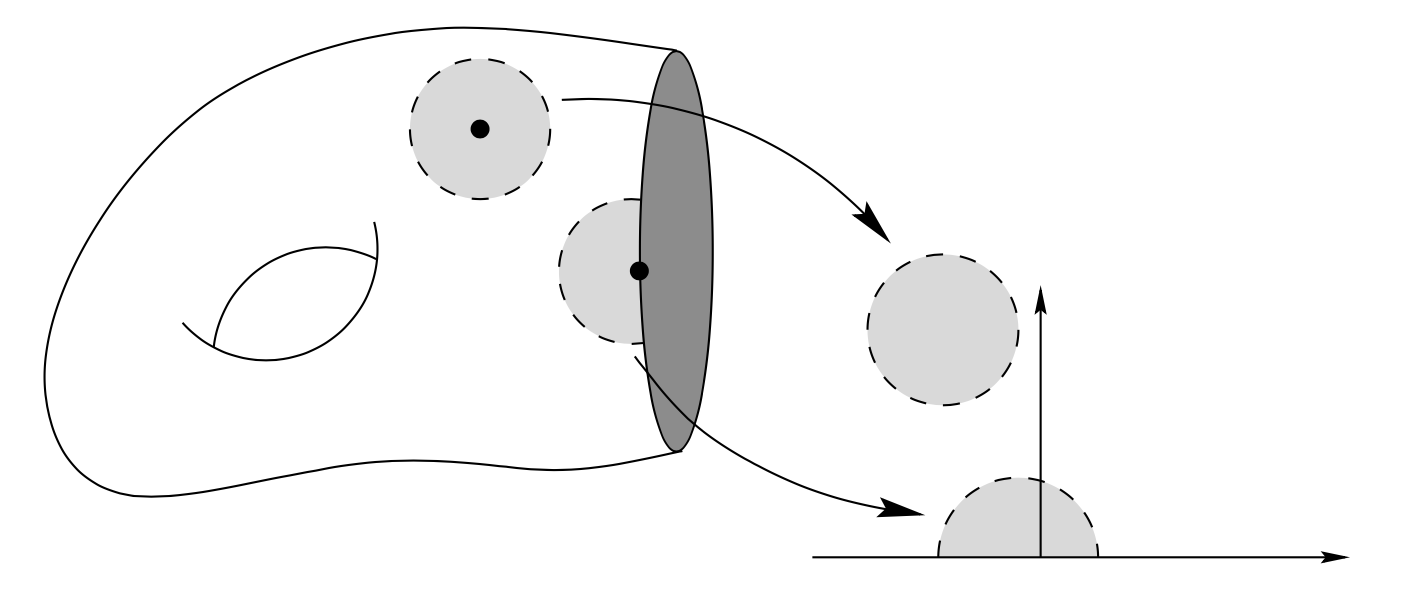
\includegraphics[scale = 0.4]{manifolds_with_boundary.png}}
\end{minipage}
\caption{\footnotesize{\textbf{A manifold with boundary \citep{lee2003introduction}}}}
\label{fig: manifolds_with_boundary}
\end{figure}

\item 
\begin{definition}
An \emph{\textbf{$n$-dimensional topological manifold with boundary}} is a \emph{second-countable Hausdorff space} $M$ in which every point has a neighborhood \emph{homeomorphic} either to \emph{an open subset} of $\bR^n$ or to a (\emph{relatively}) \emph{open subset} of $\bH^n$.
\end{definition}

\item \begin{definition}
An open subset $U \subseteq M$ together with a map $\varphi: U \rightarrow \bR^n$ that is a \emph{homeomorphism} onto an open subset of $\bR^n$ or $\bH^n$ will be called a \emph{\textbf{chart}} for $M$ , just as in the case of manifolds.
\end{definition}

\item \begin{definition}
We will call $(U, \varphi)$ an \emph{\textbf{interior chart}} if $\varphi(U)$ is an \emph{open subset} of $\bR^n$ (which includes the case of an open subset of $\bH^n$ that does not intersect $\partial\,\bH^n$), and a \emph{\textbf{boundary chart}} if $\varphi(U)$ is an open subset of $\bH^n$ such that $\varphi(U) \cap \partial\,\bH^n \neq \emptyset$. 

A \emph{boundary chart} whose image is a set of the form $B_r(x) \cap \bH^n$ for some $x \in \partial\,\bH^n$ and $r > 0$ is called a \emph{\textbf{coordinate half-ball}}.
\end{definition}

\item \begin{definition}
A point $p \in M$ is called an \emph{\textbf{interior point}} of $M$ if it is in the \emph{domain of some interior chart}. It is a \emph{\textbf{boundary point}} of $M$ if it is in the domain of a \emph{boundary chart} that sends $p$ to $\partial\,\bH^n$. The \emph{\textbf{boundary}} of $M$ (the set of all its boundary points) is denoted by $\partial\,M$; similarly, its \emph{\textbf{interior}}, the set of all its interior points, is denoted by $\text{Int}\,M$
\end{definition}

\item It follows from the definition that each point $p \in M$ is either an interior point or a
boundary point. But it cannot be simultaneously an interior point for some chart and a boundary point for another chart.

\item \begin{theorem} (\textbf{Topological Invariance of the Boundary}) \citep{lee2003introduction} \\
If $M$ is a topological manifold with boundary, then each point of $M$ is either a boundary point or an interior point, \textbf{but not both}. Thus $\partial\,M$ and $\text{Int}\, M$ are \textbf{disjoint sets} whose union is $M$.
\end{theorem}

\item A manifold with boundary may have nonempty boundary in this new sense, irrespective of whether it has a boundary \emph{as a subset }of some other topological space. There is a difference between the terms \emph{\textbf{topological boundary}} and \emph{\textbf{manifold boundary}}.

\item Note that, despite their name, \emph{\textbf{manifolds with boundary are not in general manifolds}}, because boundary points do not have locally Euclidean neighborhoods. Moreover, a manifold with boundary might have \emph{\textbf{empty boundary}} -- there is nothing in the definition that requires the boundary to be a nonempty set. 

On the other hand, \emph{\textbf{a manifold is also a manifold with boundary}}, whose boundary is empty. Thus, every manifold is a manifold with boundary, but a manifold with boundary is a manifold if and only if its boundary is empty.

\item We will often use redundant phrases such as \emph{\textbf{manifold without boundary}} if we wish to emphasize that we are talking about a manifold in the original sense, and \emph{\textbf{manifold with or without boundary}} to refer to a manifold with boundary if we wish emphasize that the boundary might be empty.

\item In the literature, you will also encounter the terms \emph{\textbf{closed manifold}} to mean a \emph{compact manifold without boundary}, and \emph{\textbf{open manifold}} to mean a \emph{noncompact manifold without boundary}.

\item \begin{proposition}
Let $M$ be a topological $n$-manifold with boundary.
\begin{enumerate}
\item $\text{Int}\, M$ is an \textbf{open subset} of $M$ and a topological n-manifold \textbf{without boundary}.
\item $\partial\,M$ is a \textbf{closed subset} of M and a \textbf{topological $(n - 1)$-manifold without boundary}.
\item $M$ is a topological manifold if and only if $\partial\,M = \emptyset$.
\item If $n = 0$,then $partial\,M = \emptyset$ and $M$ is a $0$-manifold.
\end{enumerate}
\end{proposition}

\item  The topological properties of manifolds that we proved earlier in the chapter have
natural extensions to manifolds with boundary, with essentially the same proofs as in the manifold case.
\begin{proposition}
Let $M$ be a topological $n$-manifold with boundary.
\begin{enumerate}
\item $M$ has a countable basis of \textbf{precompact} coordinate balls and \textbf{half-balls}.
\item $M$ is \textbf{locally compact}.
\item $M$ is \textbf{paracompact}.
\item $M$ is \textbf{locally path-connected}.
\item $M$ has \textbf{countably many components}, each of which is an open subset of $M$ and a connected topological manifold with boundary.
\item The \textbf{fundamental group} of $M$ is countable.
\end{enumerate}
\end{proposition}
\end{itemize}

\subsection{Smooth Structures on Manifolds with Boundary}
\begin{itemize}
\item \begin{definition}
Now let $M$ be a topological manifold with boundary. As in the manifold case, a \emph{\textbf{smooth structure}} for $M$ is defined to be a \emph{maximal smooth atlas} -- a collection of charts whose domains cover $M$ and whose transition maps (and their inverses) are smooth in the sense just described. With such a structure, $M$ is called a \emph{\textbf{smooth manifold with boundary}}. 
\end{definition}

\item Every smooth manifold is automatically a smooth manifold with boundary (whose boundary is empty).

\item \begin{definition}
Just as for smooth manifolds, if $M$ is a smooth manifold with boundary, any chart in the given smooth atlas is called a \emph{\textbf{smooth chart}} for $M$. \emph{\textbf{Smooth coordinate balls, smooth coordinate half-balls, and regular coordinate balls}} in $M$ are defined in the obvious ways. 

In addition, a subset $B \subseteq M$ is called a \emph{\textbf{regular coordinate half-ball}} if there is a smooth coordinate half-ball 
$B' \supseteq \overline{B}$ and a \emph{smooth coordinate map} $\varphi: B' \rightarrow \bH^n$ such that for some positive real numbers $0< r < r'$,
\begin{align*}
\varphi(B) = B_{r}(0)\cap \bH^{n}, \quad \varphi(\overline{B}) = \overline{B_{r}}(0)\cap \bH^{n}, \quad \varphi(B') = B_{r'}(0)\cap \bH^{n}.
\end{align*}
\end{definition}

\item One important result about smooth manifolds that \emph{\textbf{does not extend directly}} to smooth manifolds \emph{with boundary} is the construction of smooth structures on finite products. Because a product of half-spaces $\bH^n \times \bH^m$ is not itself a half-space, \emph{\textbf{a finite product of smooth manifolds with boundary cannot generally be considered as a smooth manifold with boundary}}.

\item \begin{proposition}
Suppose $M_1 ,\ldots, M_k$ are smooth manifolds and $N$ is a smooth manifold with boundary. Then $M_1 \times \ldots \times M_k \times N$ is a smooth manifold with boundary, and $\partial\,(M_1 \times \ldots \times M_k \times N) = M_1 \times \ldots \times M_k \times \partial\,N$.
\end{proposition}

\item \begin{theorem} (\textbf{Smooth Invariance of the Boundary}) \citep{lee2003introduction}\\ 
Suppose $M$ is a smooth manifold with boundary and $p \in M$. If there is some smooth chart $(U, \varphi)$ for $M$ such that $\varphi(U) \subseteq \bH^n$ and $\varphi(p) \in \partial\,\bH^n$, then the same is true for \textbf{every smooth chart} whose domain contains $p$.
\end{theorem}
\end{itemize}

\newpage
\bibliographystyle{plainnat}
\bibliography{book_reference.bib}
\end{document}